\begin{figure*}[t]
\centering
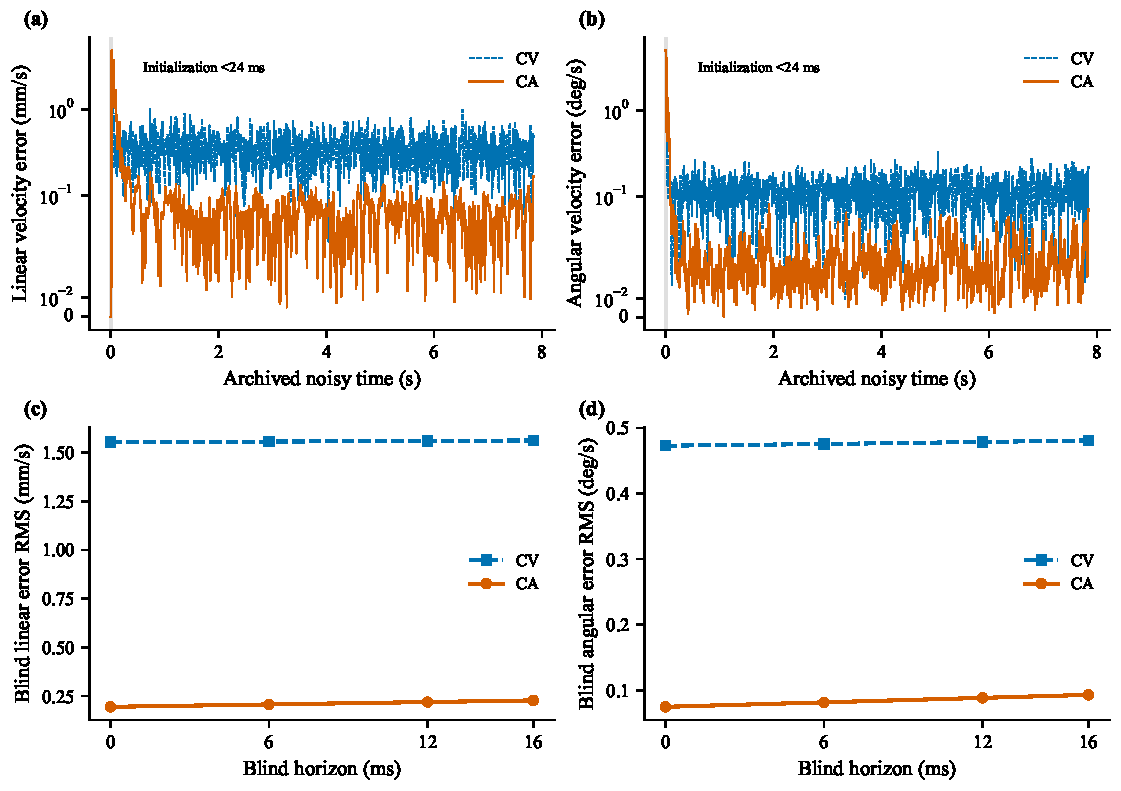
\includegraphics[width=\textwidth]{f1_causal_errors.pdf}
\caption{CV denotes the original constant-velocity estimator; CA is the new 18-state local-acceleration estimator. (a,b) World-frame geometric-origin linear and angular velocity error norms on archived R03\_V2\_S01, all times retained; gray marks invalid initialization before 24 ms. Symmetric-log axes use linear thresholds 0.05 mm/s and 0.05 deg/s. (c,d) Euclidean norm-RMS of blind errors on the synthetic bias\_noise held-out interval [2,6] s, after causal [0,2) s warmup. Forecasts assimilate no future observations. Endpoint truncation leaves 667/666/665/664 origins for horizons 0/6/12/16 ms, matched between methods. These are correlated samples, not independent trials.}
\end{figure*}

\begin{figure*}[t]
\centering
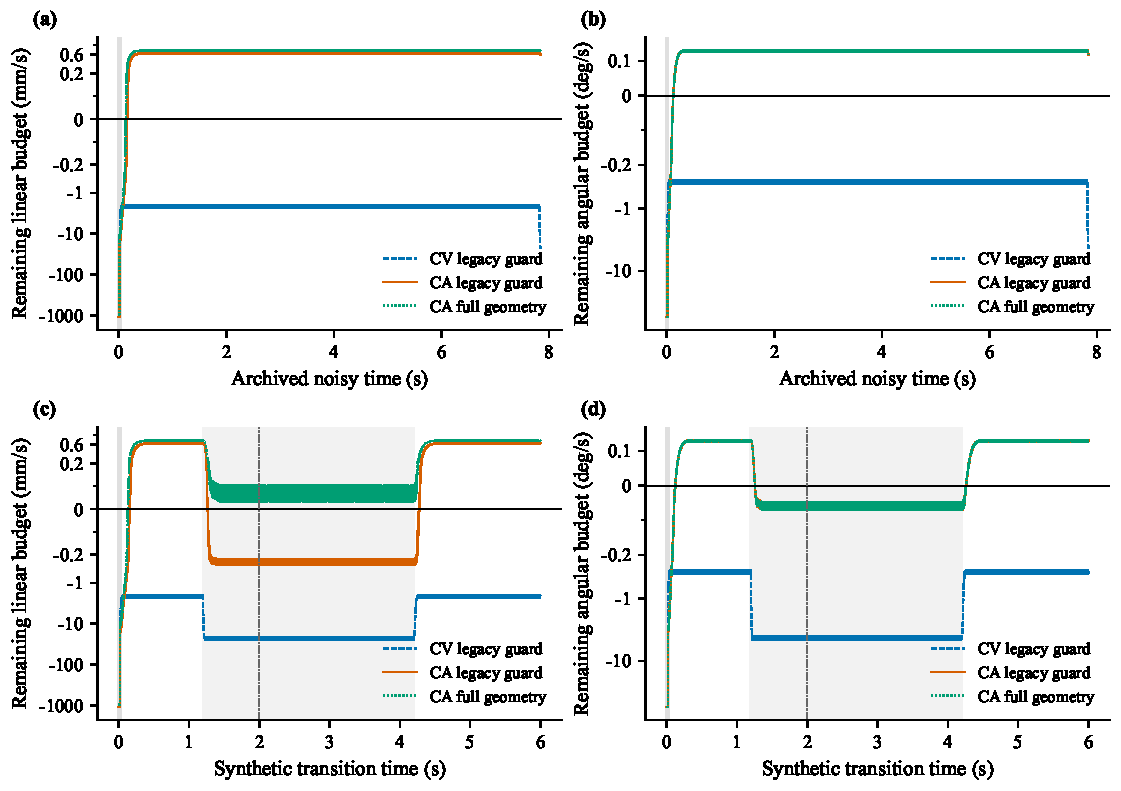
\includegraphics[width=\textwidth]{f2_guard_budget.pdf}
\caption{(a,b) Archived R03\_V2\_S01; (c,d) synthetic bias\_noise over [0,6] s, with [0,2) causal warmup before the dash-dot line and [2,6] held-out scoring. Gray at the origin marks invalid initialization before 24 ms; the wider light band marks prescribed synthetic contact process mode from 1.2 to 4.2 s, not measured robot contact. Remaining budget uses unchanged legacy 3sigma formulas; dotted CA full geometry is a diagnostic and does not replace the guard. Symmetric-log linear thresholds are 0.2 mm/s and 0.2 deg/s. Negative budget leaves no tracking reserve. Positive linear budget alone does not imply feasibility: angular budget can remain negative. R03 actual guard calls = 0; all these checks are counterfactual necessary conditions.}
\end{figure*}

\begin{figure*}[t]
\centering
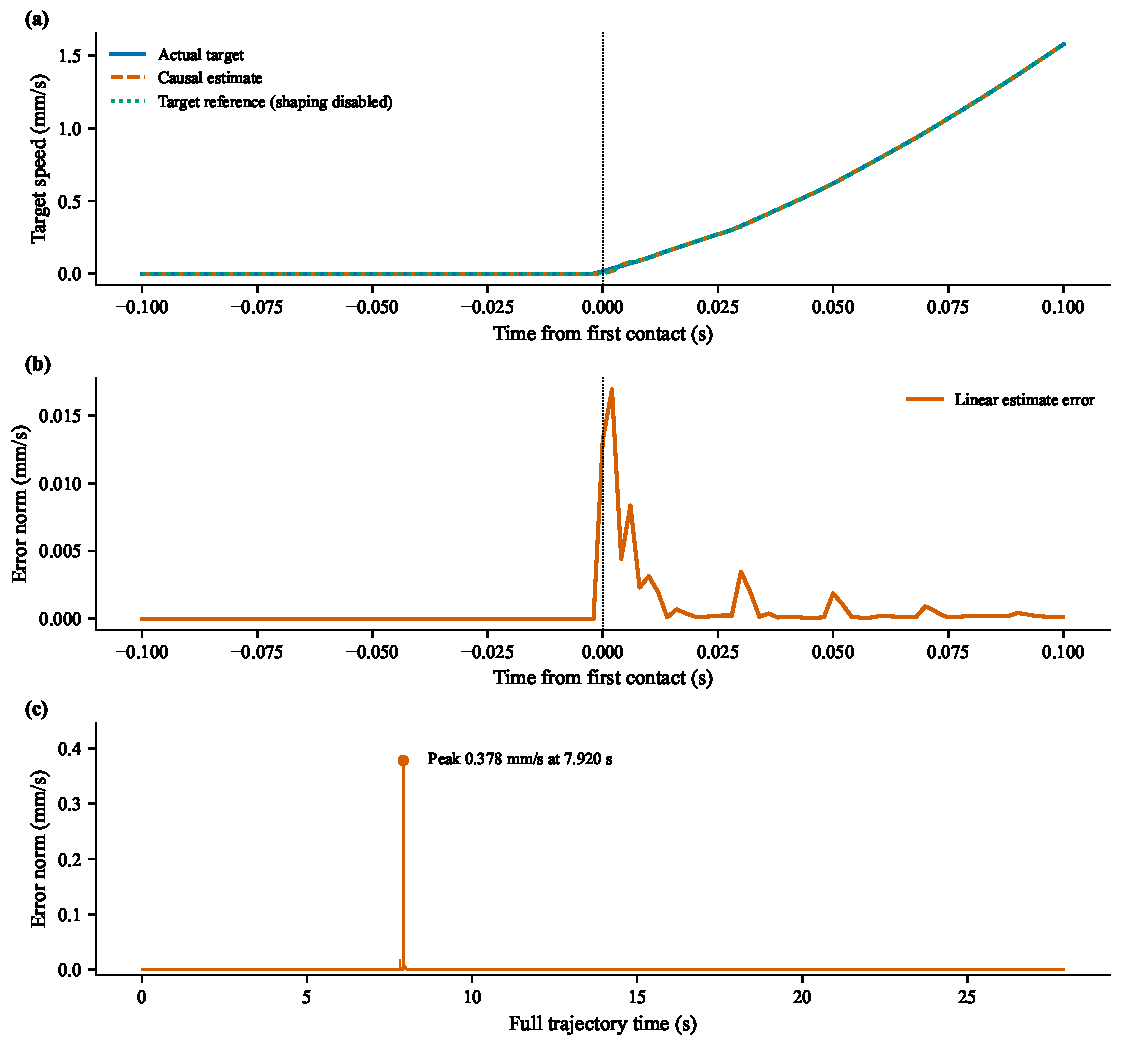
\includegraphics[width=\textwidth]{f3_contact_motion.pdf}
\caption{Corrected E0\_C2 first intended geometric contact (intentional contact count becomes positive, not a nonzero-force criterion) plus/minus 100 ms, fixed before looking at outcomes. All three curves describe world-frame target geometric-origin speed norms. This unchanged baseline has reference shaping disabled: the target reference copies the causal estimate, so those curves coincide; it is not the flange path. Panel (b) retains the contact estimation spike. Panel (c), added during result review to expose the larger latch-transition spike just outside the fixed contact window, shows every valid sample over the full trajectory and labels the maximum. This is a diagnostic presentation amendment, not a changed task-evaluation window. If the recorded prefix ends within this interval, the window is truncated there. Missing current estimates or references at an exception endpoint are left absent, never extrapolated.}
\end{figure*}

\begin{figure*}[t]
\centering
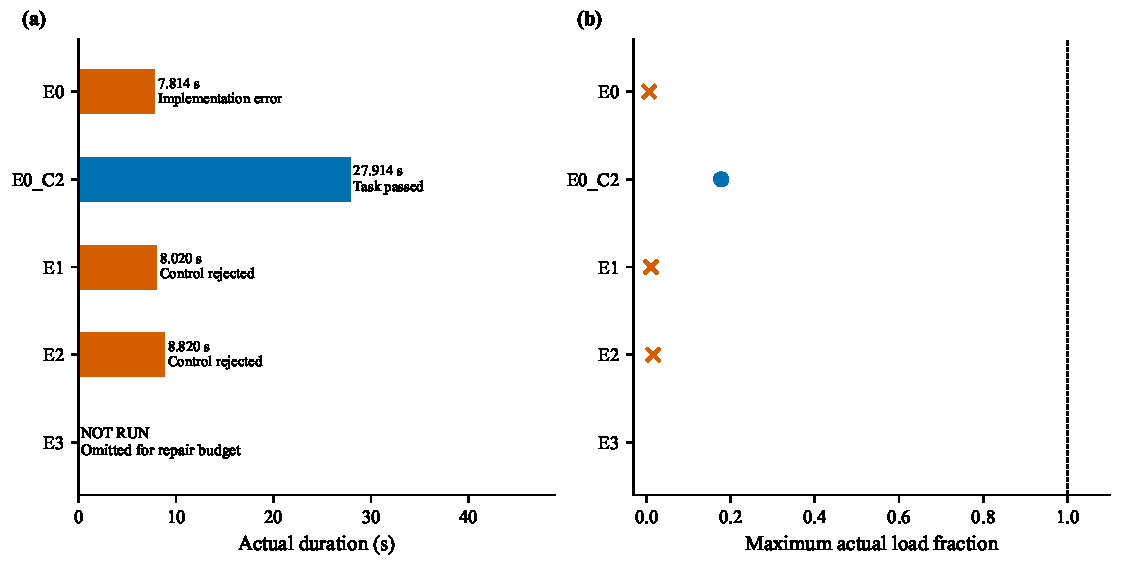
\includegraphics[width=\textwidth]{f4_task_outcomes.pdf}
\caption{Planned conditions and repair attempts: E0 and E0\_C2 are two attempts at the same ideal condition. Bars show actual duration, markers peak actual load fraction with the unchanged limit at one. Blue circles require full duration, the final detumbling gate and no recorded safety violation; orange crosses indicate failure. Row text distinguishes implementation failure and control rejection. NOT RUN is reserved for absent ledger attempts, with E3 omitted for the repair budget; a missing summary is labelled separately. Early-stop final two-second windows remain NOT\_EVALUATED.}
\end{figure*}